\section{Browser Behaviors on HTTPS Errors}
%There are many community standards for certificate validation,
%    for example,
%    RFC 5246, RFC 6125, and RFC 5280.
%    The certificate validation in browser
%    is more than a  literal replication of Internet standards protocols.
%    It needs to balance security, standards, and user experiences.
\subsection{Goal and Methodology}
Our goal is to build a test harness that is able to determine whether a web browser reports HTTPS security warning for a variety of different kinds of HTTPS errors.

we generate our own root certificate and install it so that the web browser trusts it.
    This allows us to then generate and sign intermediate and leaf certificates as we wish.
We implement out test as follows: for each test,
    (1)generates a unique DNS name,
    (2) uses OpenSSL to generate a test certificate that are syntactically well-formed but may violate one of the certificate constraints and internal dependencies that a valid certificate must satisfy.
    (3)generate an Nginx server configuration for the test.
Thus, each test has a dedicated DNS name and Nginx instance to serve the certificate chain.
    We create a web page to present the browser certificate validation results.
    Thus, We can record whether the HTTPS security warning is triggered by such a combination of a test certificate and a HTTPS implementation.
    In our experiment, All connections to the web server is encrypted and authenticated using TLS 1.2.

The evaluated browsers are Chrome 67.0.3396.99, Firefox 62.0, Edge 42.17134.1.0, and IE 11.0.9600.17031 on Windows 10. The results are summarized in Table I.
\begin{table*}[htbp]
\centering
\begin{tabular}{p{2.2cm}|l|cccc}
\toprule
\multicolumn{2}{c|}{\multirow{2}{*}{HTTPS Errors}} & \multicolumn{4}{l}{Risk Levels of Browser Security Warnings} \\ \cline{3-6}
\multicolumn{2}{c|}{} & Chrome & Firefox & Edge & IE \\ \midrule[1pt]
\multirow{12}{*}{\begin{tabular}[c]{@{}c@{}}Basic Certificate \\ Validation Error\end{tabular}} & Untrusted self-signed server certificate & B & B & B & B \\
 & Untrusted root CA certificate & B & B & B & B \\
 & Incomplete Certificate Chain & B & B & B & B \\
 & Expired & B & B & B & B \\ \cline{2-6}
 & Revoked(CRL) & Secure & Secure & C & C \\
 & Revoked(OCSP) & Secure & C & C & C \\
 & Revoked(Chrome CRLset) & C & Secure & Secure & Secure \\ \cline{2-6}
 & Insufficient key length (RSA512) & B & B & B & C \\
 & Insufficient key length (RSA1024) & Secure & Secure & Secure & Secure \\
 & Insufficient key length (ECC160) & D & D & D & D \\ \cline{2-6}
 & Weak signature(SHA-1) & B & B & Secure & Secure \\
 & Weak signature(MD5) & B & B & Secure & Secure \\ \midrule[1pt]
\multirow{17}{*}{\begin{tabular}[c]{@{}c@{}}Certificate Extension \\ Validation Error\end{tabular}} & server certificate &  &  &  &  \\
 & ~~incorrect CA falg & Secure & B & Secure & Secure \\
 & CA certificate &  &  &  &  \\
 & ~~incorrect CA falg & C & - & C & C \\
 & ~~correct CA flag, incorrect PathLenConstraint & C & Secure & C & B \\ \cline{2-6}
 & server certificate &  &  &  &  \\
 & ~~no extended key usage, correct key usage & Secure & Secure & Secure & Secure \\
 & ~~no extended key usage, incorrect key usage & Secure & C & Secure & Secure \\
 & ~~no extended key usage, no key usage & Secure & Secure & Secure & Secure \\
 & ~~correct extended key usage, correct key usage & Secure & Secure & Secure & Secure \\
 & ~~correct extended key usage, incorrect key usage & Secure & Secure & Secure & Secure \\
 & ~~correct extended key usaget, no key usage & Secure & Secure & Secure & Secure \\
 & ~~incorrect extended key usage, correct key usage & C & C & C & C \\
 & ~~incorrect extendedKeyUsage error, incorrect key usage & C & C & C & C \\
 & ~~incorrect extendedKeyUsage, no key usage & C & C & C & C \\
 & CA certificate &  &  &  &  \\
 & ~~key usage error & C & C & C & C \\ \midrule[1pt]
\multirow{11}{*}{\begin{tabular}[c]{@{}c@{}}Name Validation \\ Error\end{tabular}} & domain name complete mismatch & B & B & B & B \\
 & www mismatch & B & B & B & B \\
 & out-of-wildcard-scope subdomain error & B & B & B & B \\ \cline{2-6}
 & SAN and CN &  &  &  &  \\
 & ~~correct SAN, no CN & Secure & Secure & Secure & Secure \\
 & ~~correct SAN, incorrect CN & Secure & Secure & Secure & Secure \\
 & ~~incorrect SAN, no CN & B & B & B & B \\
 & ~~incorrect SAN, correct CN & B & B & B & B \\
 & ~~incorrect SAN, incorrect CN & B & B & B & B \\
 & ~~no SAN, incorrect CN & B & B & B & B \\
 & ~~no SAN, correct CN & B & Secure & Secure & Secure \\ \midrule[1pt]
\multirow{13}{*}{\begin{tabular}[c]{@{}c@{}}HTTPS Security \\ Enhancement Error\end{tabular}} & HPKP: private store &  &  &  &  \\
 & ~~first visit: incorrect HPKP header, second visit: correct/incorrect/no HPKP header & Secure & Secure & Secure & Secure \\
 & ~~first visit: correct HPKP header, second visit: correct HPKP header & Secure & Secure & Secure & Secure \\
 & ~~first visit: correct HPKP header, second visit: incorrect/no HPKP header & Secure & Secure & Secure & Secure \\
 & HPKP: public store &  &  &  &  \\
 & ~~first visit: incorrect HPKP header, second visit: correct/incorrect/no HPKP header & Secure & Secure & Secure & Secure \\
 & ~~first visit: correct HPKP header correct, second visit: correct HPKP heade & Secure & Secure & Secure & Secure \\
 & ~~first visit: correct HPKP header correct, second visit: incorrect/no HPKP header & B & Secure & Secure & Secure \\ \cline{2-6}
 & HSTS: not preload list &  &  &  &  \\
 & ~~some resouces over plain HTTP & A & A & A & A \\
 & ~~first visit: correct HSTS header, second visit: HTTPS error & B-\textgreater{}C & B-\textgreater{}C & B-\textgreater{}C & B-\textgreater{}C \\
 & ~~first visit: incorrect HSTS header, second visit: correct/incorrect/no HSTS header & S & S & S & S \\
 & HSTS: preload list &  &  &  &  \\
 & ~~first visit: HTTPS errors & B-\textgreater{}C & B-\textgreater{}C & B-\textgreater{}C & B-\textgreater{}C \\ \bottomrule
\end{tabular}
\end{table*}%


%\textbf{Certificate has no partial fields.}
%    A certificate may not have a Common Name or SAN field. In OpenSSL, certificates that do not fill in the above fields can also be generated and be signed.
 %   For the Common Name, some very old browsers may not support certificates without Common Name. % The Chrome browser does not support certificates without a SAN field.

\subsection{Warnings on Basic Certificate Validation Error}

\textbf{Untrusted Self-signed Server Certificate.}
    When we visit sites deploying self-signed server certificates, all four browsers display B-level (Medium-risk) warnings.
    After installing the self-signed certificates into the OS root store, Chrome, Edge, and IE consider it secure.
    However, The NSS store in Firefox does not accept self-signed certificates, and Firefox always displays B-level (Medium-risk) warnings for self-signed sever certificates.

%\textbf{Untrusted Root CA Certificate.}
%\textbf{Incomplete Certificate Chain.}
%\textbf{Expired Certificate.}
    For Untrusted Root CA Certificate, Incomplete Certificate Chain, and Expired Certificate errors,
        all four browsers display B-level (Medium-risk) warnings.

\textbf{Revoked Certificate.}
    If a revoke certificate only contains available CRL field,
        Chrome and Firefox consider it secure,
            but Edge and IE display C-level (High-risk) warnings.
    If a revoke certificate only contains available OCSP field,
        Chrome considers it secure, but Firefox,
            Edge and IE display C-level (High-risk) warnings.
    If a revoke certificate is only included in Chrome CRLset,
        Chrome displays a C-level (High-risk) warning,
            but Firefox, Edge and IE consider it secure.

%\textbf{Weak Signature Algorithm.}
\textbf{Weak Signature Algorithm.}
    For RSA 512,
        Chrome, Firefox, and Edge display B-level (Medium-risk) warnings,
            but IE display a C-level (High-risk) warning.
    For RSA 1024,
        all four browsers consider it secure.
    For ECC 160,
        all four browsers display D-level (Fatal) warnings.

%\textbf{Weak Digest Algorithm.}
\textbf{Weak Digest Algorithm.}
    For SHA-1 and MD5,
        Chrome and Firefox display B-level (Medium-risk) warnings,
            but Edge and IE consider them secure.

\subsection{Warnings on Certificate Extension Validation Error}

\textbf{Basic Constraints Extension.}
    If a server certificate is signed by a CA certificate that has a correct CA flag but does not conform to PathLenConstraint,
    Chrome and Edge display C-level (High-risk) warnings,
    Firefox consider it secure, and IE displays a B-level (Medium-risk) warning.

    If a server certificate whose CA flag is true,
    Chrome, Edge, and IE consider it secure,
    and Firefox displays a B-level (Medium-risk) warning.

    If a server certificate is signed by a certificate whose CA flag is false,
     Chrome, Edge, and IE display C-level (High-risk) warnings.
     Firefox's NSS root store does not accept a certificate whose CA flag is false, so we does test the Firefox for this HTTPS error.

\textbf{Key Usage Extension and Extended Key Usage Extension.}
    If a server certificate has Extended key usage field including serverAuth, no matter what the key usage is,
        all the four browsers consider it secure.
    If a server certificates has Extended key usage field not including serverAuth, no matter what the key usage is,
        all the four browsers display C-level (High-risk) warnings.
    If a server certificates does not have Extended key usage field, and its key usage field is correct or does not have key usage field,
        all the four browsers consider it secure.
    If a CA certificate has incorrect key usage field,
        all the four browsers display C-level (High-risk) warnings.


\subsection{Warnings on Name Validation Error}
    For domain name complete mismatch, www mismatch, and out-of- wildcard scope subdomain error,
    all four browsers display B-level (Medium-risk) warnings.

    For correct SAN, no matter what the CN is, all the four browsers consider it secure.
    For incorrect SAN, no matter what the CN is, all the four browsers display B-level (Medium-risk) warnings.
    If the server certificate does not have SAN field, and the CN field is incorrect, all the four browsers display B-level (Medium-risk) warnings.
    If the server certificate does not have SAN field, and the CN field is incorrect,
    Chrome displays a B-level (Medium-risk) warning,
            but Firefox, Edge, and IE consider it secure.

\subsection{Warnings on HTTPS Security-Enhancement Error}


The site's certificate must first be trusted by the browser, including server authentication and certificate/certificate chain verification. We first pin the sha256 value of the intermediate CA and any other sha256 value into the header, and the browser will cache the two sha256 values ??and verify them in the next access within the cache effective time. If the two sha256 values ??of the pin are in the same certificate chain, they will not be cached and will not prompt any errors.

If the next time the certificate issued by the site is valid and the certificate is in the pin list, the HPKP cache will be refreshed, including the SHA-256 value of the pin and the cache validity period, whichever comes first. If the intermediate CA of a certificate chain that a webmaster plans to replace is not in the current pin, you should keep using the original certificate or the alternate certificate and change the value of the other pin until the longest cache time, you can safely delete the old certificate's Pin.

In a site with HPKP cache and in effect, if the certificate received when accessing the site is a certificate in the public certificate store, and the certificate chain is not in the pin, it will be reported by the browser, but can be ignored. If the visited site is in a private certificate store, ie a self-signed certificate chain, no errors will be reported even if the certificate does not comply with the HPKP policy, and the HPKP settings cache will not be updated.

The cache of the HPKP policy has no relationship with the storage area where the certificate is located. If the certificate is legal in the browser and does not conflict with the pin in the cache, the sha256 value of the self-signed certificate chain is also stored in the pin of the HPKP policy.

When the site has the HSTS header set and is not in the preloaded list, the first visit to the site does not force https access. When the local browser has the HSTS setting cache, the browser will make a jump inside the browser when accessing the http site without initiating an HTTP network request.

\begin{figure}[htbp]
\centerline{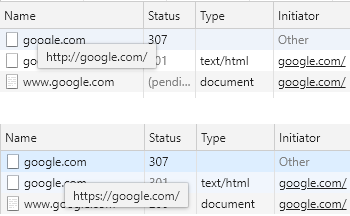
\includegraphics{Figure/fig5.png}}
\caption{Network requests to access a site with HSTS.}
\label{fig}
\end{figure}

The cache obtained by the browser through the HSTS response header is stored in the dynamic HSTS, and the site in the preloaded list is in the static storage area, which cannot be modified after the browser is compiled. However, the HSTS policy is stored in two areas and has no effect on the validity of the settings.

The HSTS policy only takes effect in the risk alert that the browser can skip. It will block the option to ignore the error, and the browser will also prompt "Cannot continue browsing due to the HSTS policy." For low-risk prompts (Level A), the browser can still access the site normally, and there will be an exclamation point prompt, which is no different from the prompt without the HSTS policy. Naturally, there is no change to the risk alert (Level C) that could not be skipped.

